\documentclass[a4paper,10pt,fleqn]{jarticle}
\usepackage{graphicx}
\usepackage{amssymb}
\usepackage{amsmath}
\usepackage{ascmac}
\usepackage{setspace}
\usepackage{float}
\usepackage{slashbox}
\usepackage[dvips,usenames]{color}
\usepackage{colortbl}
\usepackage{eclbkbox}
\usepackage{indent}
\definecolor{bl}{gray}{0.8}
\definecolor{myred}{rgb}{1,0,0} 
\definecolor{mygreen}{rgb}{0,1,0} 
\definecolor{myblue}{rgb}{0,0,1} 
\definecolor{mycyan}{rgb}{0,1,1} 
\definecolor{mymagenta}{rgb}{1,0,1} 
\definecolor{myyellow}{rgb}{1,1,0} 
%--余白の設定
\setlength{\topmargin}{20mm}
\addtolength{\topmargin}{-1in}
\setlength{\oddsidemargin}{20mm}
\addtolength{\oddsidemargin}{-1in}
\setlength{\evensidemargin}{15mm}
\addtolength{\evensidemargin}{-1in}
\setlength{\textwidth}{170mm}
\setlength{\textheight}{254mm}
\setlength{\headsep}{0mm}
\setlength{\headheight}{0mm}
\setlength{\topskip}{0mm}
\makeatletter
\def\@oddhead{}
\def\@evenhead{}
\def\@evenfoot{\normalfont\rmfamily\hfil---\,\thepage\,---\hfil}
\def\@oddfoot{\normalfont\rmfamily\hfil---\,\thepage\,---\hfil}
\def\ps@titlepage{\let\@oddhead\@empty}
\def\ps@titlepage{\let\@evenhead\@empty}
\makeatother
\begin{document}
\pagenumbering{arabic}
\section{Rとは}
1996年に登場した,オープンソースでフリーの統計解析向け言語及び開発実行環境であり,最新バージョンは3.2.0 (2015/4/16 release).Linux,Windows,OSX で利用可能である.似た言語では S言語があり,Rが開発される前にAT\&Tベル研究所によって開発された統計処理言語である.

Rではさまざまな構造のデータを保持でき,記法がC言語に似ている為,習得が大変容易である.コントリビュータによって用意されるパッケージも豊富で,その数は5000個以上である.

\section{Rをインストールしよう}
まず,{\tt http://www.r-project.org/} にアクセスし,左サイドバーの CRAN をクリックすると,CRAN のミラーサーバを選択する画面が表示されるので,なるべく日本のミラーサーバを選択する.日本でのミラーサーバは神戸教育大学・筑波大学・統計数理研究所に存在している.オススメは統計数理研究所(Institute of Statistical Mathematics, Tokyo).

ミラーサーバにアクセスし,OSを選択する.以下の作業は,リリースされている最新バージョンによって表示が多少異なる.
また,インストール時の画像は R3.0.2 のものである.

\subsection{Windowsの場合}
\underline{Download R for Windows} → \underline{base} → \underline{Download R 3.2.0 for Windows} (62 megabytes, 32/64 bit) の順にクリックし,インストーラをダウンロードする.

\includegraphics[width=2cm]{img/windows/win001.eps} ダウンロードしたインストーラを起動し,以下のダイアログを進めていく.

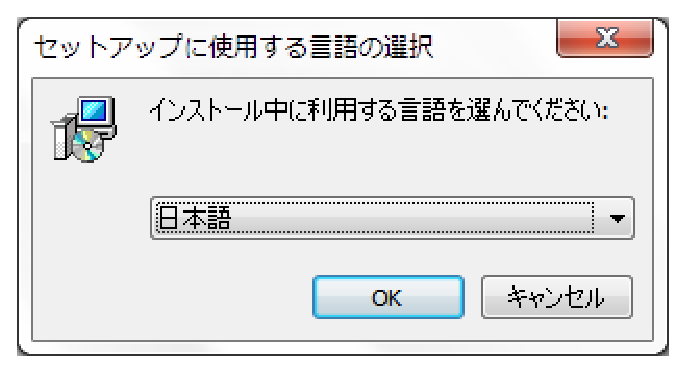
\includegraphics[width=6cm]{img/windows/win002.eps}\hspace{0.8em} 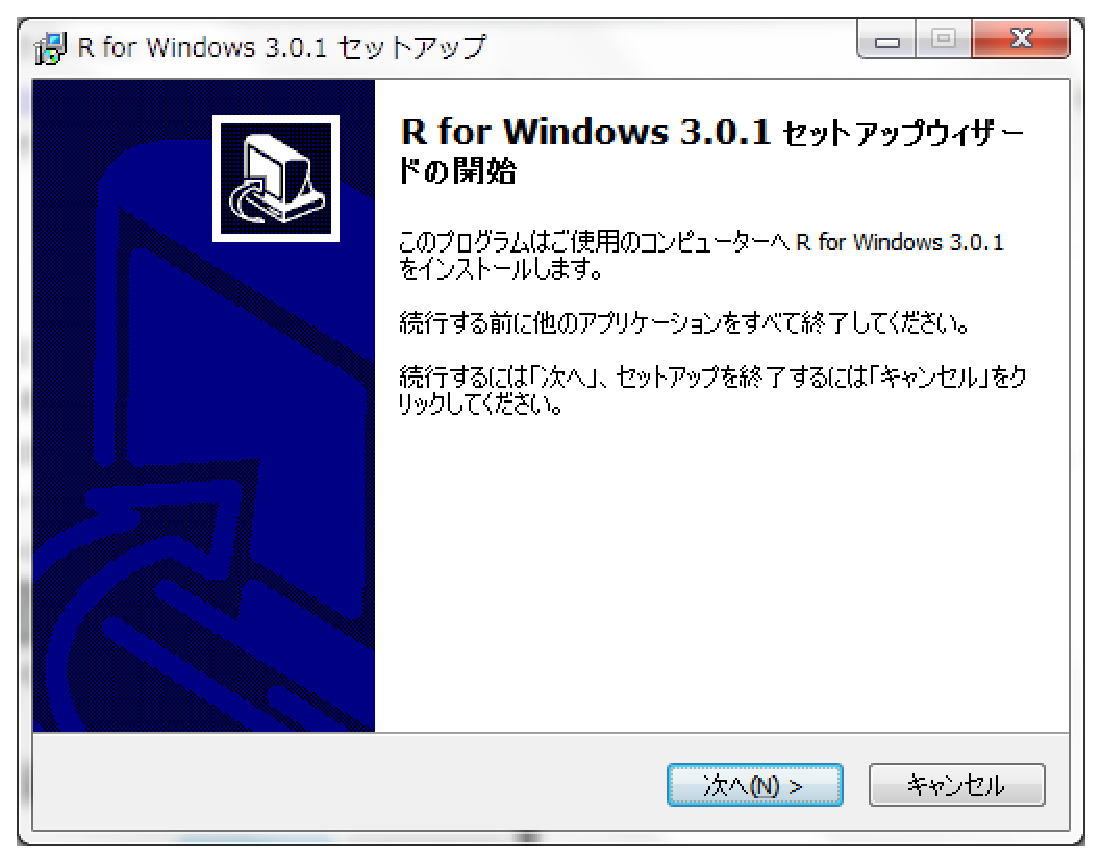
\includegraphics[width=8cm]{img/windows/win003.eps}\\

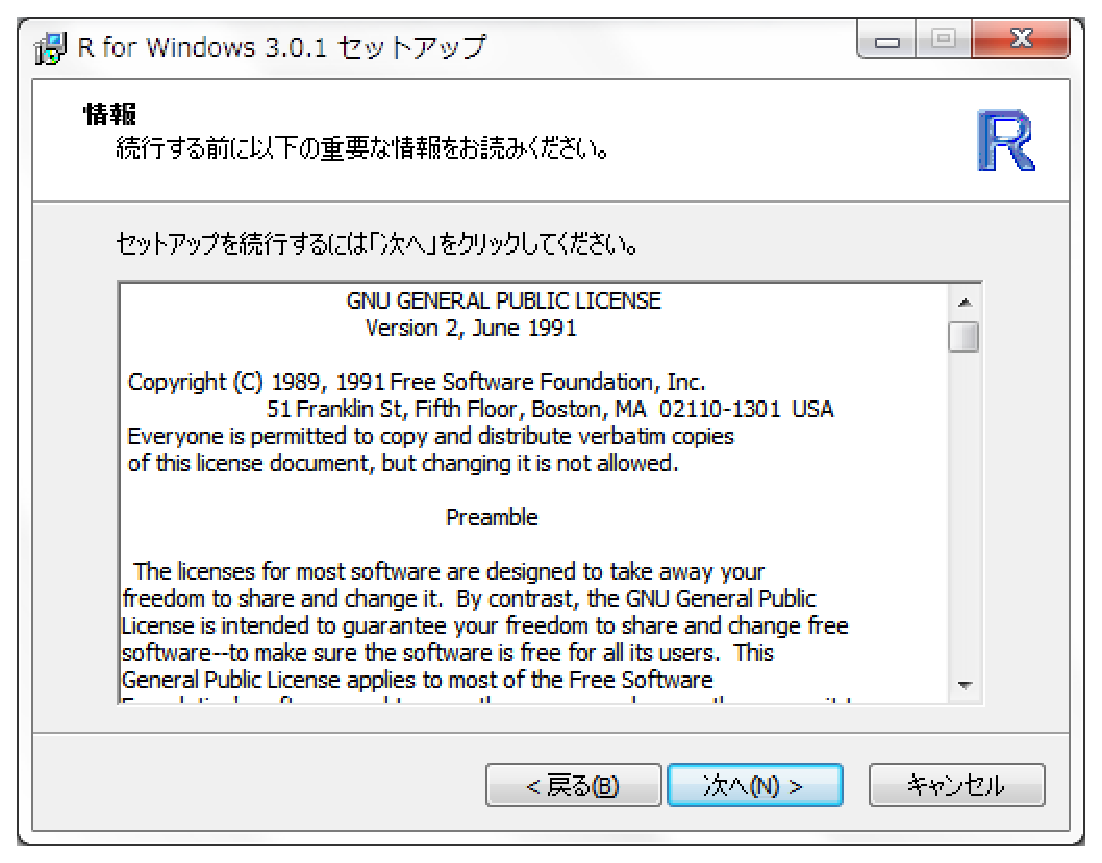
\includegraphics[width=8cm]{img/windows/win004.eps}\hspace{0.8em} 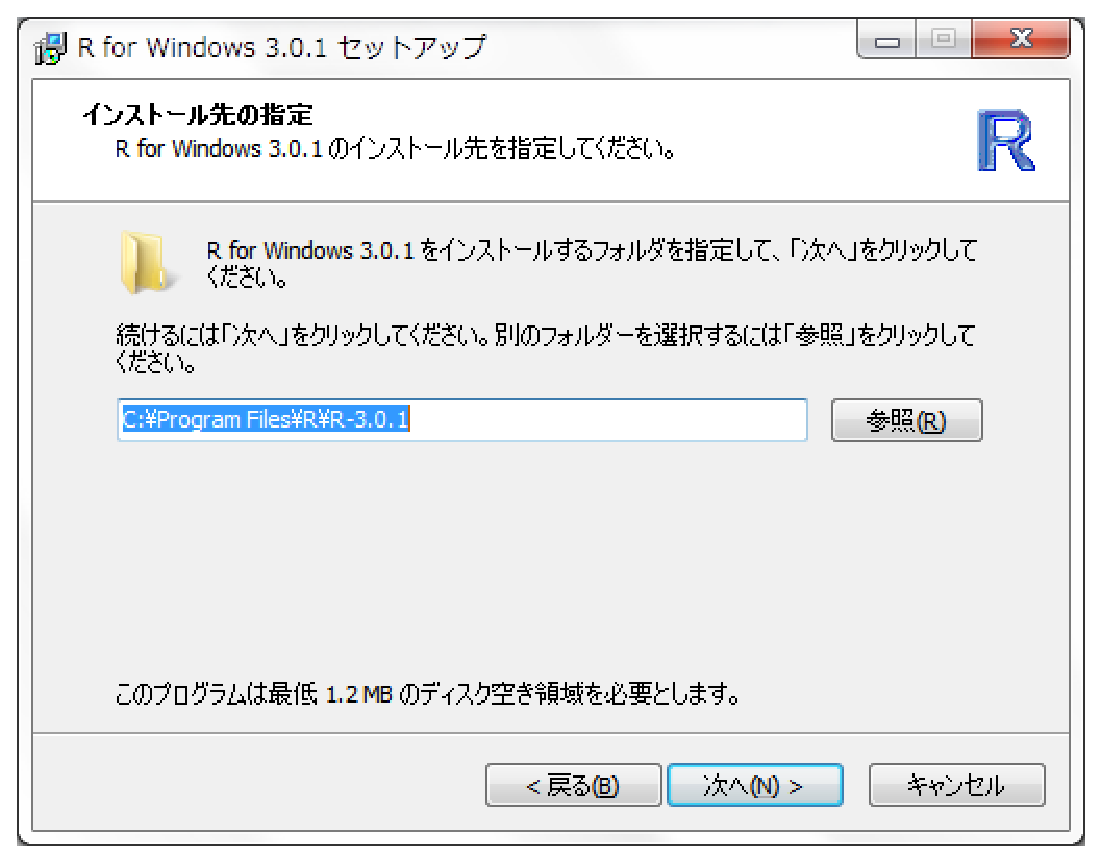
\includegraphics[width=8cm]{img/windows/win005.eps}\\

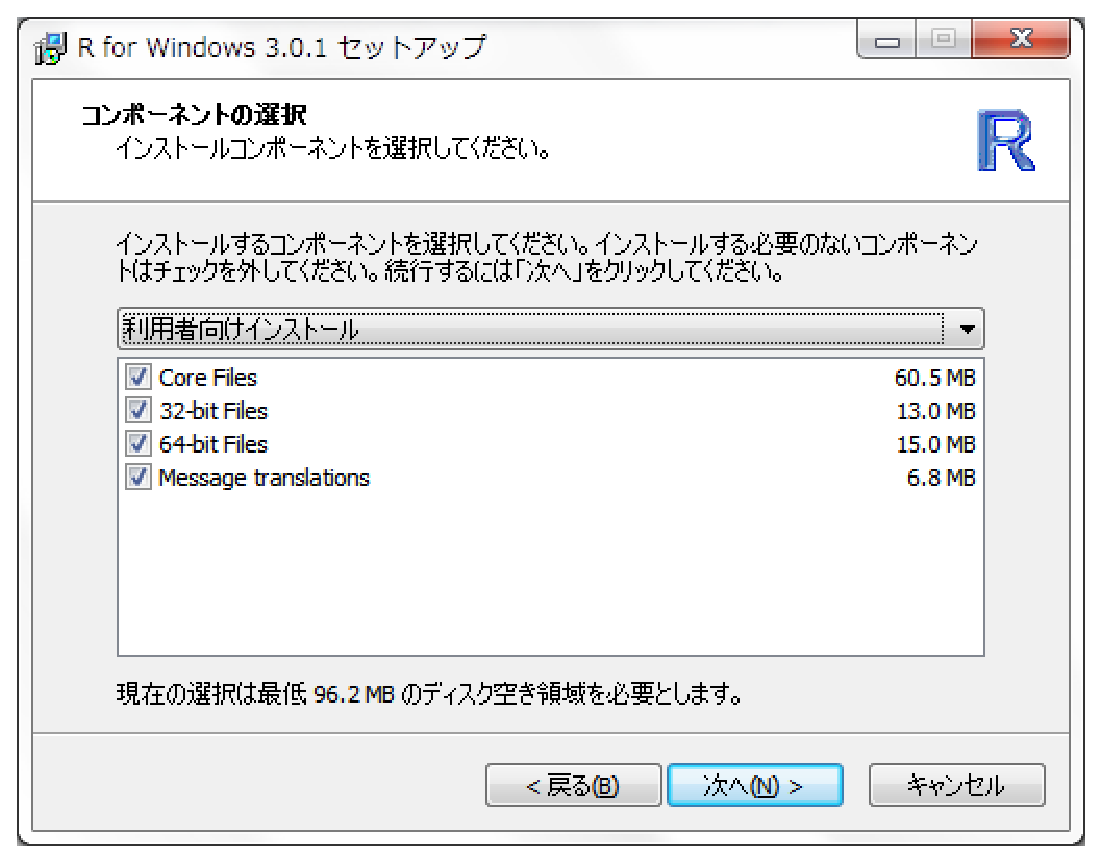
\includegraphics[width=8cm]{img/windows/win006.eps}\hspace{0.8em} 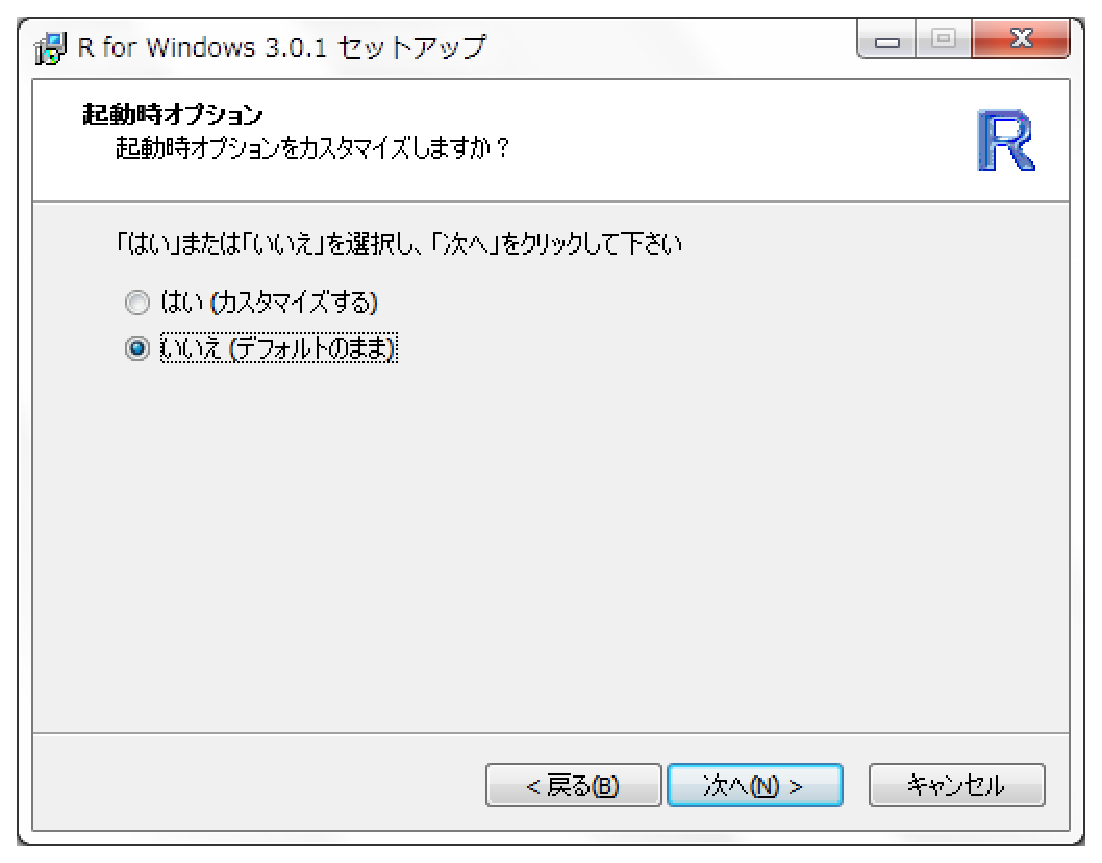
\includegraphics[width=8cm]{img/windows/win007.eps}\\

\includegraphics[width=8cm]{img/windows/win008.eps}\hspace{0.8em} 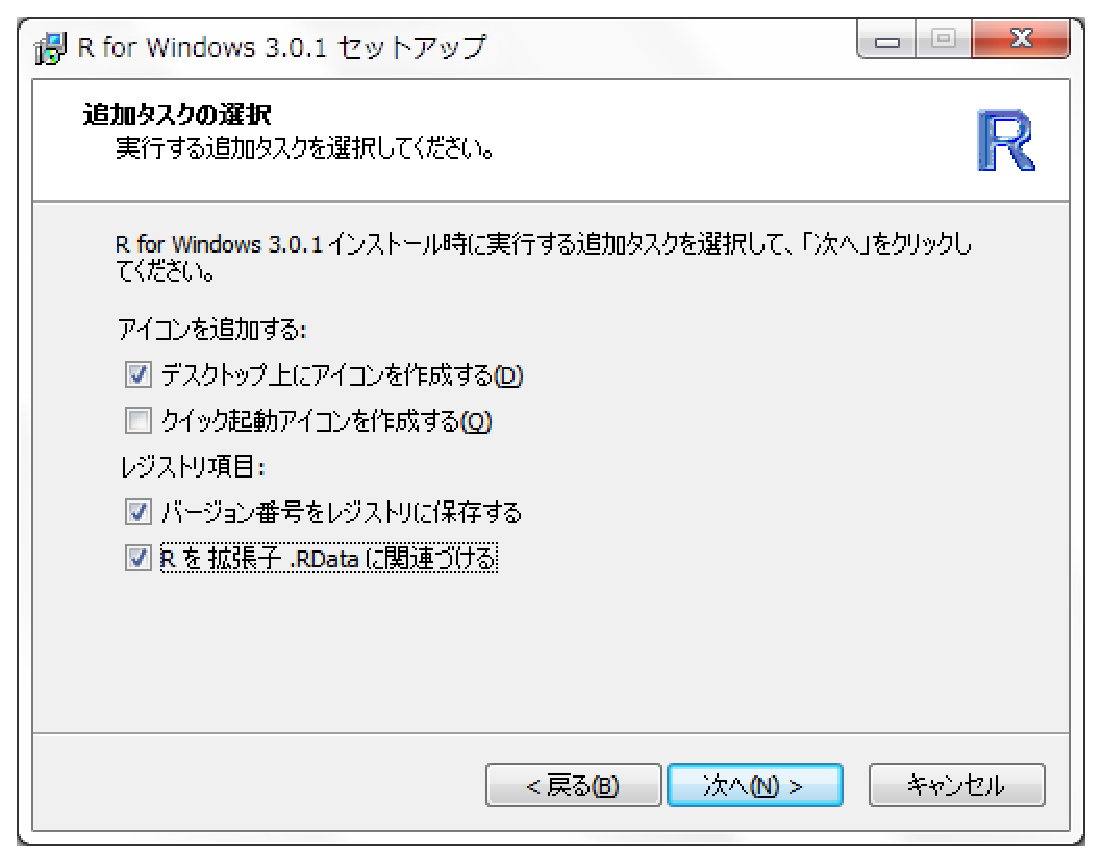
\includegraphics[width=8cm]{img/windows/win009.eps}\\

\includegraphics[width=8cm]{img/windows/win010.eps}\hspace{0.8em} 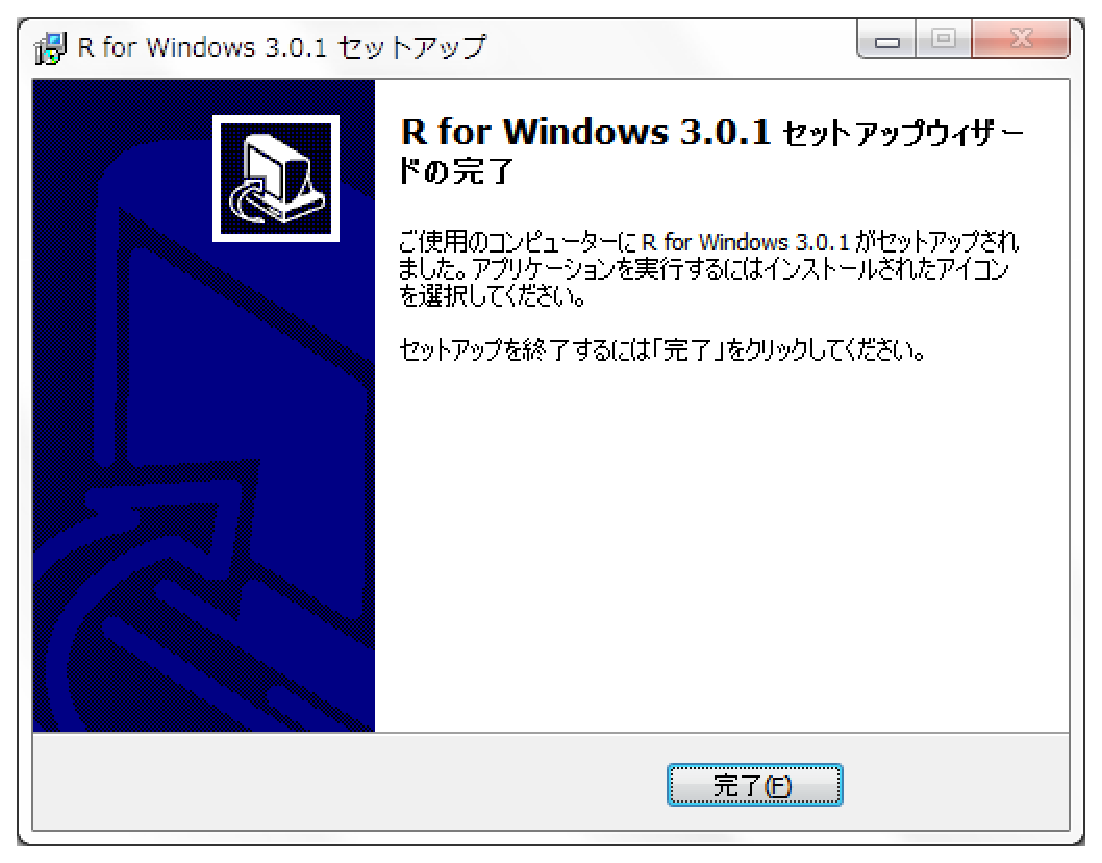
\includegraphics[width=8cm]{img/windows/win011.eps}\\

以上でインストールは完了する.\\

デスクトップに作成されたショートカット 
\includegraphics[width=1.7cm]{img/windows/win012.eps}より起動する.
\subsection{OSX (Mac)の場合}
\underline{Download R for (Mac) OS X} → \underline{R-3.2.0.pkg} の順にクリックし,インストーラをダウンロードする.\\
OS が古い場合は\underline{R-3.1.3-snowleopard.pkg}を用いてインストールする.
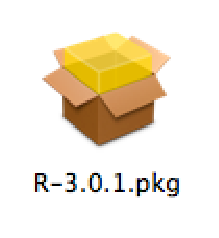
\includegraphics[width=1.8cm]{img/osx/osx001.eps} ダウンロードしたインストーラを起動し,以下のダイアログを進めていく.\\

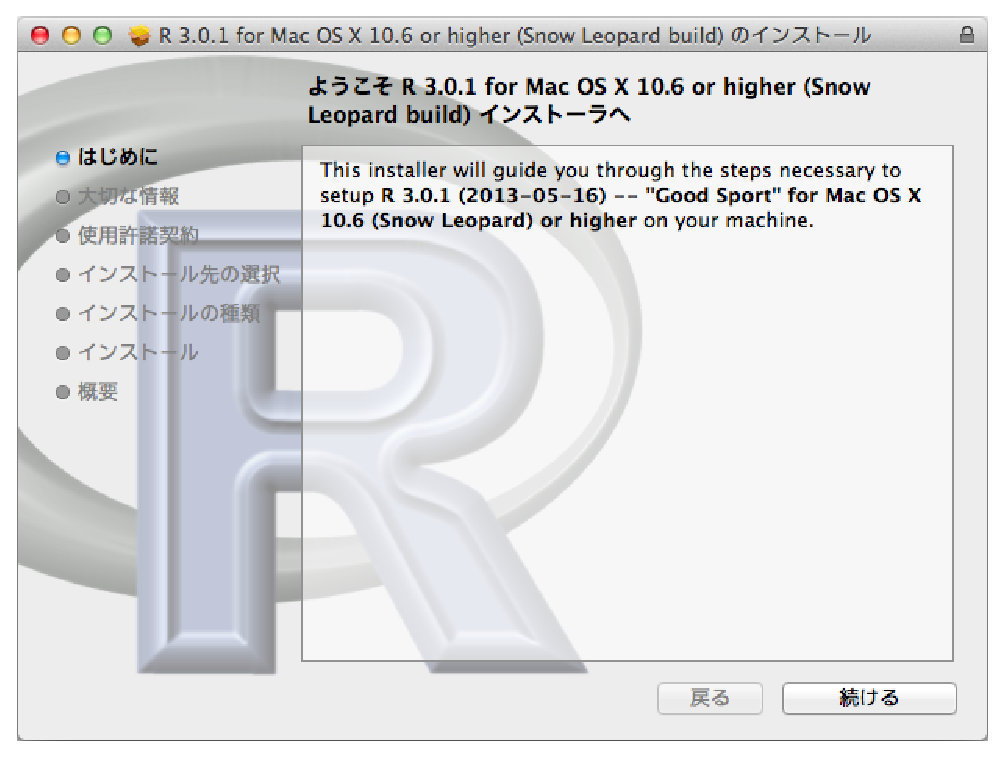
\includegraphics[width=8cm]{img/osx/osx002.eps}\hspace{0.8em} 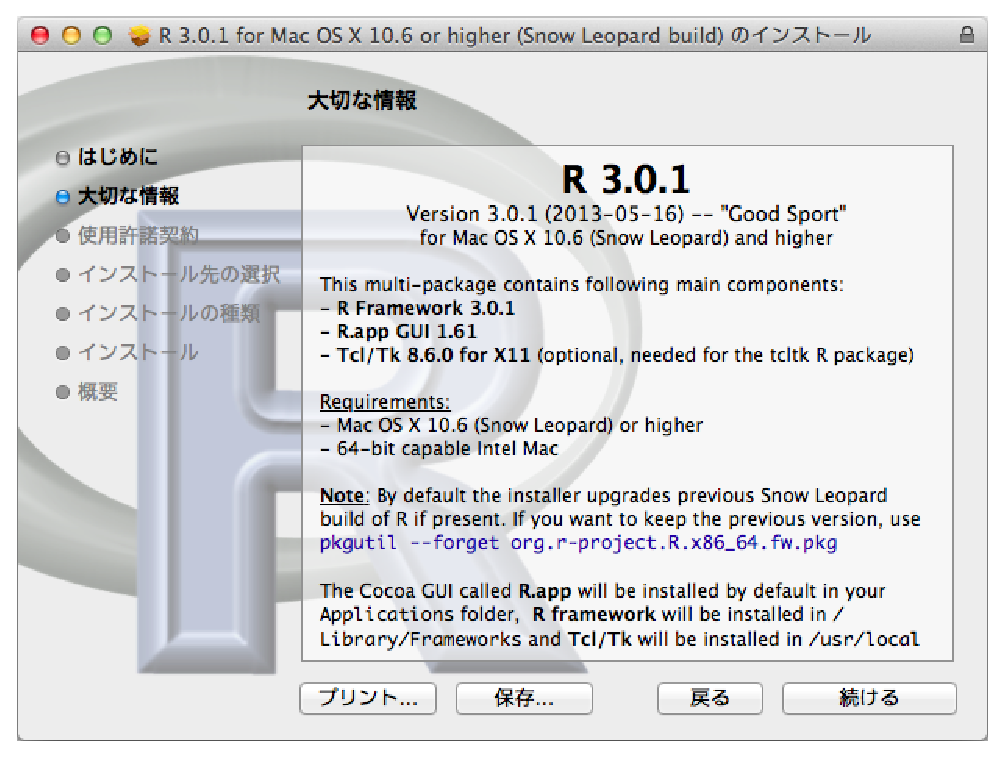
\includegraphics[width=8cm]{img/osx/osx003.eps} \\

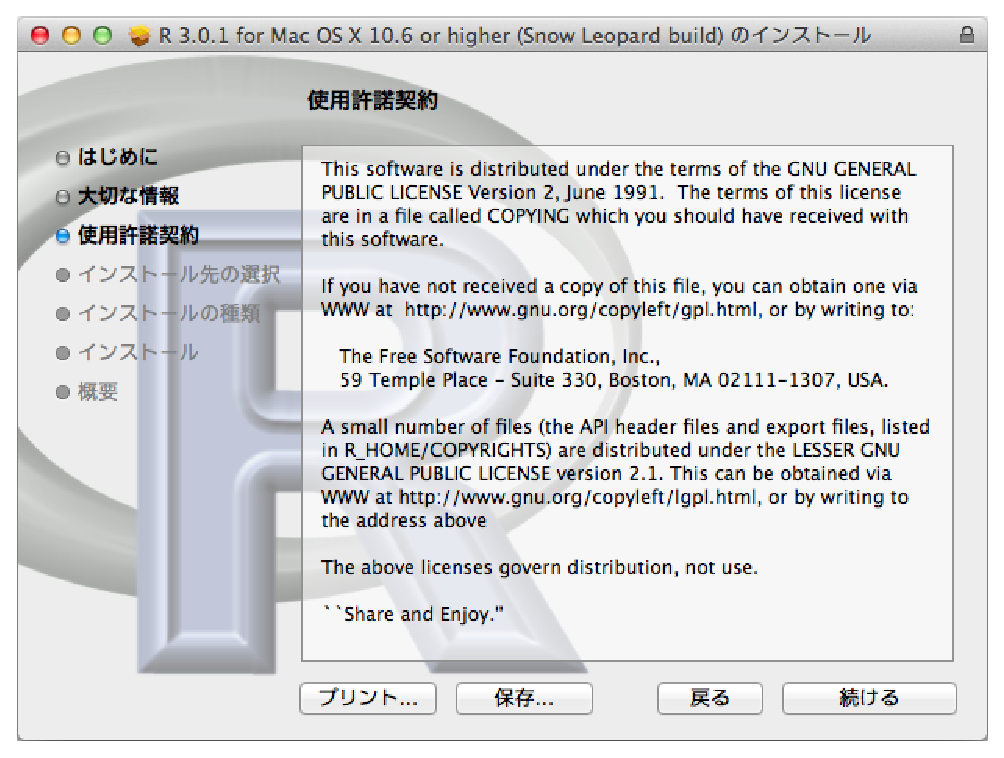
\includegraphics[width=8cm]{img/osx/osx004.eps}\hspace{0.8em} 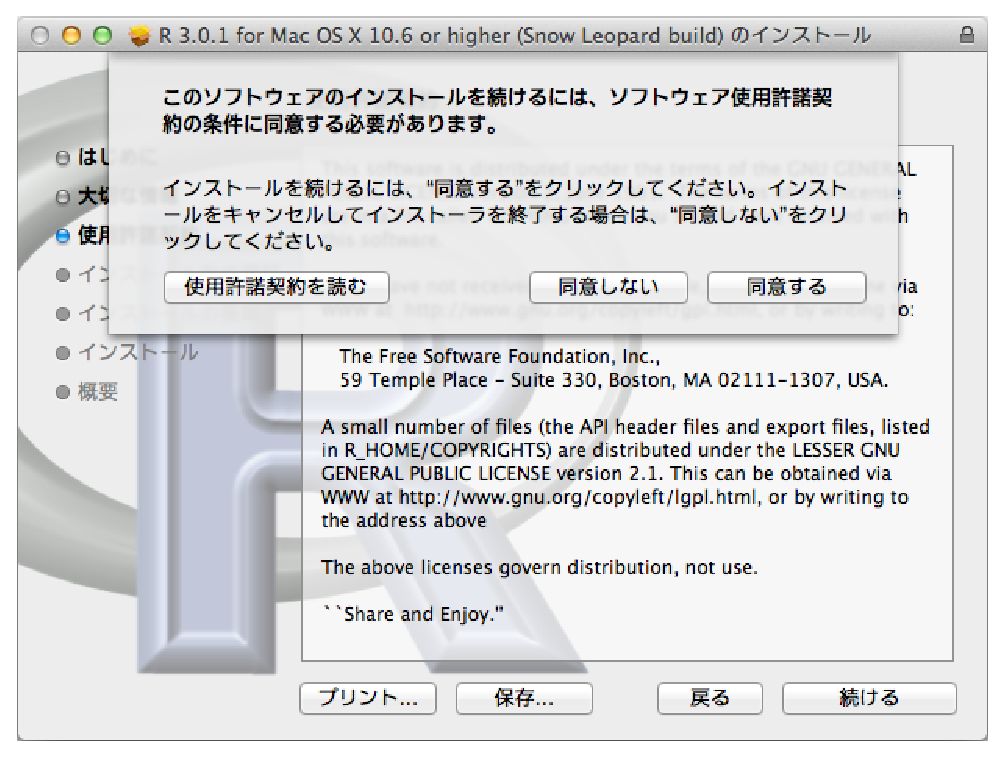
\includegraphics[width=8cm]{img/osx/osx005.eps}\\

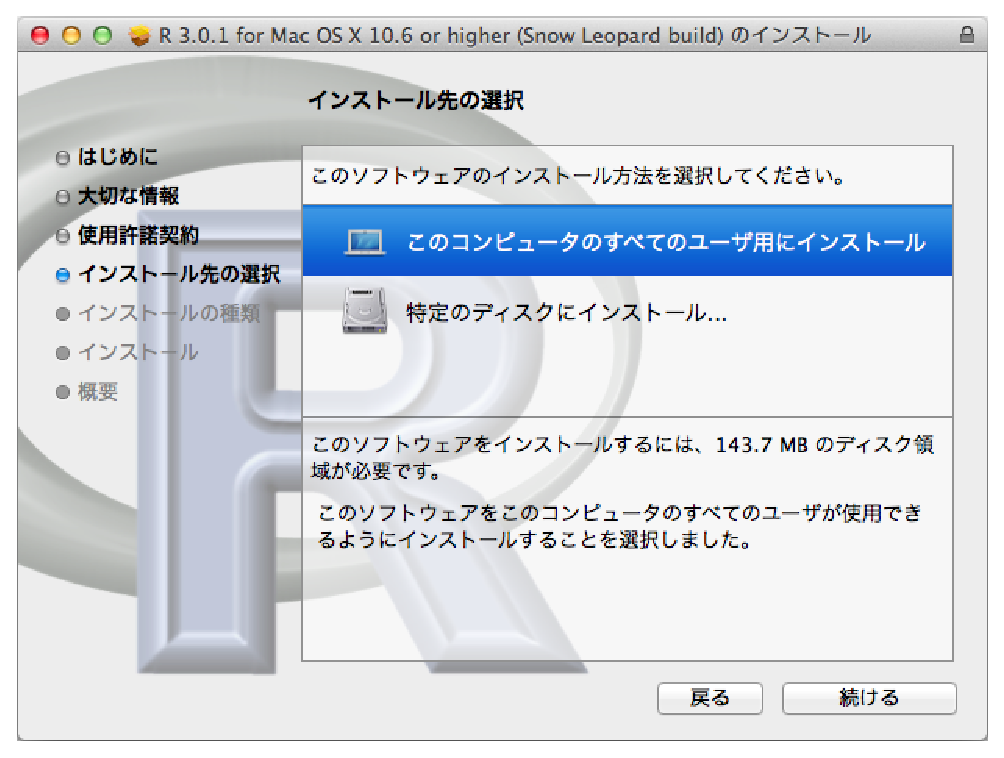
\includegraphics[width=8cm]{img/osx/osx006.eps}\hspace{0.8em} \includegraphics[width=8cm]{img/osx/osx007.eps}\\

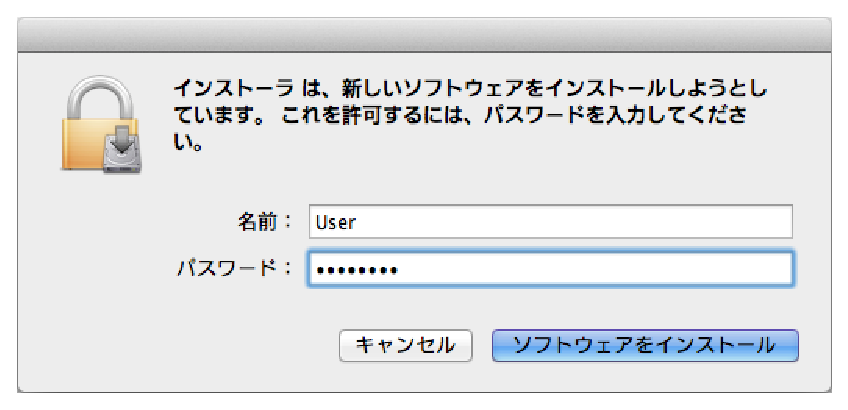
\includegraphics[width=8cm]{img/osx/osx008.eps}\hspace{0.8em} 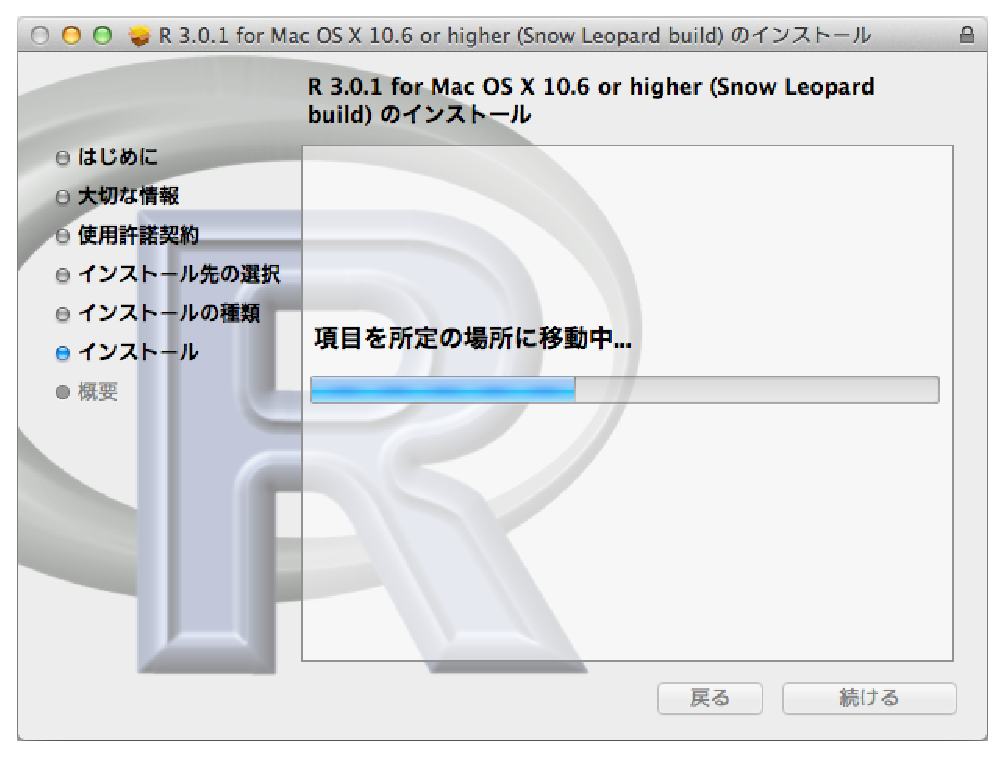
\includegraphics[width=8cm]{img/osx/osx009.eps}\\

\includegraphics[width=8cm]{img/osx/osx010.eps}\hspace{0.8em} \includegraphics[width=8cm]{img/osx/osx011.eps}\\

以上でインストールは完了する.\\

アプリケーションにある 
\includegraphics[width=1.8cm]{img/osx/osx012.eps}より起動する.
\subsection{Linuxの場合}
パッケージ管理システムでインストールが可能.\verb+apt-get+では以下の様にインストールを行う.
\begin{breakbox}
\begin{verbatim}
sudo apt-get update
sudo apt-get install r-base
\end{verbatim}
\end{breakbox}
\end{document}